\documentclass{beamer}

% For more theme options:
%/usr/share/texmf/tex/latex/beamer/base/themes/theme/compatibility
\usepackage{beamerthemelined}

% this package seems to throw an error for me. -Juneki 12/6/14
%\usepackage[usenames,dvipsnames,svgnames,table]{xcolor}
\usepackage{soul}

\usepackage{algorithm}
\usepackage[noend]{algpseudocode}
\usepackage{graphicx}
\usepackage{caption}
\usepackage{subcaption}

\usepackage{tikz-dependency}

\newcommand{\eqnref}[1]{\eqref{eqn:#1}}
%\usepackage[usenames,dvipsnames,svgnames,table]{xcolor}  % allows better color names
\usepackage{todonotes}   % insert [disable] to disable all notes
\newcommand{\Note}[4][]{\todo[author=#2,color=#3,fancyline,#1]{#4}}
\newcommand{\noteJH}[2][]{\Note[#1]{JH}{blue!40}{#2}}
\newcommand{\noteJE}[2][]{\Note[#1]{JE}{green!40}{#2}}
\newcommand{\notewho}[3][]{\Note[#1]{#2}{orange!40}{#3}}  % extra arg with miscellaneous author
\newcommand{\NoteJH}[2][]{\noteJH[inline,#1]{#2}}
\newcommand{\NoteJE}[2][]{\noteJE[inline,#1]{#2}}
\newcommand{\Notewho}[3][]{\notewho[inline,#1]{#2}{#3}}  % extra arg with miscellaneous author



\begin{document}
\title{Deriving Multi-Headed Planar Dependency Parses from Link Grammar Parses}
\author{Juneki Hong, Jason Eisner}
\date{\today}
\frame{\titlepage}

\section{Motivation}
\frame{\frametitle{Motivation}

}

\section{Multi-headed}
\frame{\frametitle{Multi-headed Dependency Parsing}

\begin{figure}
  \centering
  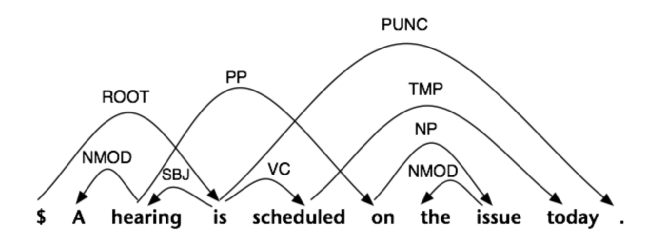
\includegraphics[width=\linewidth]{multiheaded}
  \caption{English is not completely multiheaded}
  \NoteJH{image taken from Chris Dyer's slide: http://demo.clab.cs.cmu.edu/fa2014-11711/images/0/0e/Depparsing.pdf}
\end{figure}

}


\section{Link Grammars}
\frame{\frametitle{Link Grammars}

\begin{figure}
\begin{subfigure}[b]{0.4850\textwidth}
	\begin{dependency}
		\begin{deptext}
			the \& matter \& may \& never \& even \& be \& tried \& in \& court \& . \\
			- \& n-u \& v \& e \& e \& v \& v-d \& r \& n-u \& - \\
		\end{deptext}
		\depedge[edge above, edge style = {red}]{2}{3}{S}
		\depedge[edge above, edge style = {red}]{3}{6}{I}
		\depedge[edge above, edge style = {red}]{2}{1}{D}
		\depedge[edge above, edge style = {red}]{7}{8}{MV}
		\depedge[edge above, edge style = {red}]{6}{7}{P}
		\depedge[edge above, edge style = {red}]{8}{9}{J}
		\deproot[edge above, edge style = {red}]{2}{W}
		\deproot[edge above, edge style = {red}]{7}{WV}
		\deproot[edge above, edge style = {red}]{10}{X}
		\depedge[edge above, edge style = {red}]{6}{4}{E}
		\depedge[edge above, edge style = {red}]{6}{5}{E}
	\end{dependency}
\end{subfigure}

\end{figure}
\NoteJH{figure not centered}
\NoteJH{Make the edges undirected}

}


\frame{\frametitle{Link Grammars}
\begin{figure}
\begin{subfigure}[b]{0.4850\textwidth}
	\begin{dependency}
		\begin{deptext}
			{\scriptsize DT} \& {\scriptsize NN} \& {\scriptsize MD} \& {\scriptsize RB} \& {\scriptsize RB} \& {\scriptsize VB} \& {\scriptsize VB} \& {\scriptsize IN} \& {\scriptsize NN} \& {\scriptsize .} \\
			the \& matter \& may \& never \& even \& be \& tried \& in \& court \& . \\
			- \& n-u \& v \& e \& e \& v \& v-d \& r \& n-u \& - \\
		\end{deptext}
		\deproot[edge above, edge style = {blue, dotted}]{3}{\small ROOT}
		\depedge[edge below, edge style = {red, ultra thick}]{2}{3}{S}
		\depedge[edge above, edge style = {blue, ultra thick}]{3}{2}{\small SBJ}
		\depedge[edge above, edge style = {blue, dotted}]{3}{4}{\small ADV}
		\depedge[edge above, edge style = {blue, dotted}]{3}{5}{\small ADV}
		\depedge[edge below, edge style = {red, thick}]{3}{6}{I}
		\depedge[edge above, edge style = {blue, thick}]{3}{6}{\small VC}
		\depedge[edge above, edge style = {blue, dotted}, edge unit distance =1.5ex]{3}{10}{\small P}
		\depedge[edge below, edge style = {red, thick}]{2}{1}{D}
		\depedge[edge above, edge style = {blue, thick}]{2}{1}{\small NMOD}
		\depedge[edge below, edge style = {red, thick}]{7}{8}{MV}
		\depedge[edge above, edge style = {blue, thick}]{7}{8}{\small ADV}
		\depedge[edge below, edge style = {orange, thick}]{6}{7}{P}
		\depedge[edge above, edge style = {blue, thick}]{6}{7}{\small VC}
		\depedge[edge below, edge style = {red, thick}]{8}{9}{J}
		\depedge[edge above, edge style = {blue, thick}]{8}{9}{\small PMOD}
		\deproot[edge below, edge style = {red, dotted}]{2}{W}
		\deproot[edge below, edge style = {orange, ultra thick, dotted}]{7}{WV}
		\deproot[edge below, edge style = {red, dotted}]{10}{X}
		\depedge[edge below, edge style = {red, dotted}]{6}{4}{E}
		\depedge[edge below, edge style = {red, dotted}]{6}{5}{E}
	\end{dependency}
\end{subfigure}

\end{figure}


}


\section{ILP}
\frame{\frametitle{Integer Linear Programming}

\NoteJH{Will the audience know about ILP?}


}


\section{ILP Model}
\frame{\frametitle{Integer Linear Programming Model}

\NoteJH{Take from the paper.}

}



\section{Experiments and Results}
\frame{\frametitle{Experiments and Results}

}



\section{Conclusions}
\frame{\frametitle{Conclusions}

}



\end{document}
